%!TEX root = paper.tex
%
% PyClaw
%
% Lead currently:  David Ketcheson
%

\subsection{\pyclaw} \label{sec:pyclaw}
\pyclaw is an object-oriented Python package that provides a convenient way
to set up problems and call the algorithms of \clawpack.  It grew
from what was initially a set of data structures and file IO routines that are
used by the other \clawpack codes and by \visclaw.  These routines were released in
an early form in later 4.x versions of \clawpack.  Those releases also
included a fully-functional implementation of the 1D classic algorithm
in pure Python. That implementation still exists in \pyclaw and is useful
for understanding the algorithm.

The current release of \pyclaw includes access to the classic algorithms as well
as the high-order algorithms introduced in \sharpclaw \cite{2013_sharpclaw} (i.e., WENO
reconstruction and Runge--Kutta integrators) and can be used on large
distributed-memory parallel machines.  For the latter capability, \pyclaw
relies on PETSc \cite{petsc-user-ref}.
Lower-level code (whatever gets executed
repeatedly and needs to be fast) from the earlier Fortran Classic and \sharpclaw
codes is automatically wrapped at install time using \texttt{f2py}.

Recent applications of \pyclaw include studies of laser light trapping by moving
refractive index perturbations \cite{sanroman_thesis}, instabilities of weakly nonlinear detonation
waves \cite{faria2015qualitative}, and effective dispersion of nonlinear waves via diffraction in
periodic materials \cite{2015_diffractons}.  Two of these are depicted in
\cref{fig:pyclaw-apps}.

\begin{figure}
\begin{center}
\plotbox{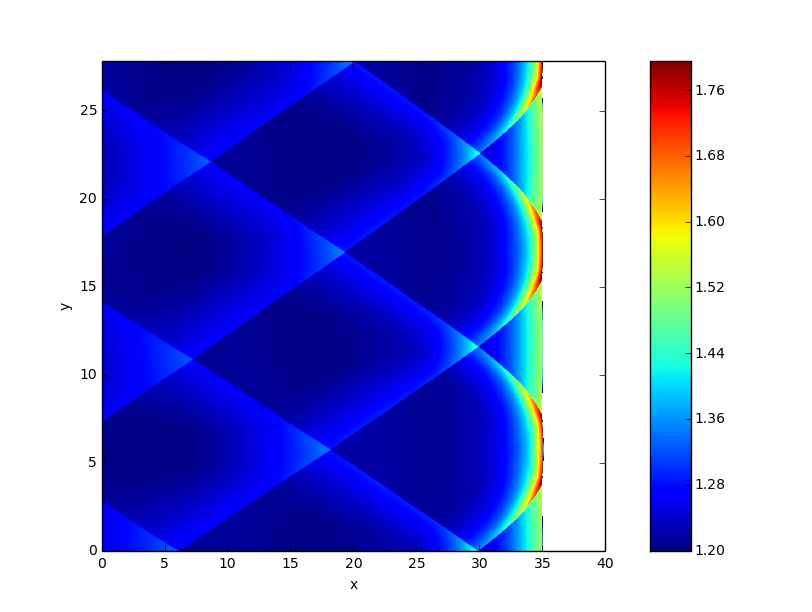
\includegraphics[height=0.35\textwidth]{detonation.png}}\hfil
\plotbox{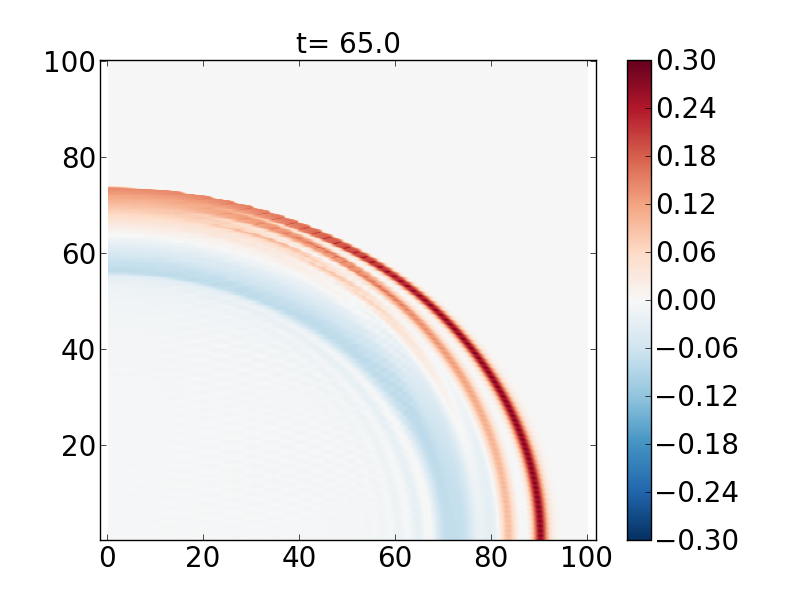
\includegraphics[height=0.35\textwidth]{diffractons.png}}
\end{center}
\caption{\label{fig:pyclaw-apps}
Left: A two-dimensional detonation wave solution of the reactive Euler equations,
showing transverse shocks that arise from instabilities; see \cite{faria2015qualitative}.
Right: Dispersion of waves in a layered medium with matched impedance and periodically-varying
sound speed; see \cite{2015_diffractons}.}
\end{figure}


\subsubsection{Librarization and extensibility}
Scientific software is easier to use, extend, and integrate with other tools
when it is designed as a library \cite{Brown:2015cj}.  \clawpack has always been
designed to be extensible, but \pyclaw takes this further in several ways.
First, it is distributed via a widely-used package management system,
\texttt{pip}. Second, the default installation process (``\texttt{pip install
clawpack}'') provides the user with a fully-compiled code and does not require
setting environment variables.  Like other \clawpack packages, \pyclaw provides
several ``hooks'' for users to plug in custom routines (for instance, to specify
boundary conditions). In \pyclaw, these routines -- including the Riemann solver
itself -- are selected at run-time, rather than at compile-time.  These routines
can be written directly in Python, or (if they are performance-critical) in a
compiled language (like Fortran or C) and wrapped with one of the many available
tools.  Problem setup (including things like initial conditions, algorithm
selection, and output specification) is also performed at run-time, which means
that researchers can bypass much of the slower code-compile-execute-post-process
cycle. It is intended that \pyclaw be easily usable within other packages
(without control of \texttt{main()}).

\subsubsection{Python geometry}
\pyclaw includes Python classes for describing collections of structured grids
and data on them. These classes are also used by the other codes and
\visclaw, for post-processing.  A mesh in \clawpack always consists of a set of
(possibly mapped) tensor-product
grids (interval, quadrilateral, or hexahedral), also referred to as patches.
At present, \pyclaw solvers operate only on a single patch, but the
geometry and grids already incorporate multi-patch
capabilities for visualization in \amrclaw and \geoclaw.

\subsubsection{\pyclaw solvers}

PyClaw includes an interface to both the Classic solvers (already
described above) and those of \sharpclaw \cite{ketcheson2012pyclaw}.
\sharpclaw uses a traditional method-of-lines approach to achieve
high-order resolution in space and time.  Spatial operators are
discretized first, resulting in a system of ODEs that is then solved
using Runge--Kutta or linear multistep methods.  The spatial
derivatives are computed using a weighted essentially non-oscillatory
(WENO) reconstruction from cell averages, which suppresses spurious
oscillations near discontinuities.  The WENO routines in \sharpclaw
were generated by PyWENO\footnote{\url{http://github.com/memmett/PyWENO}}, which
is a standalone package
that generates WENO routines.

The default time stepping routines in \sharpclaw are strong stability
preserving (SSP) Runge--Kutta methods of order two to four.
Some of the methods use extra stages in order to allow more efficient
time stepping with larger CFL numbers.
Time stepping in \sharpclaw has recently been augmented to include
linear multistep methods with variable step size.  These methods use
a time step size selection that ensures the strong stability preserving
property, as described in \cite{ssp_lmm_vss}.

\subsubsection{Parallelism}
\pyclaw includes a distributed parallel backend that uses PETSc through
the Python wrapper {\tt petsc4py}.  The parallel code uses the same low-level
routines without modification.  In the high-level routines, only a few hundred
lines of Python code deal explicitly with parallel communication, in order to
transfer ghost cell information between subdomains and to find the global
maximum CFL number in order to adapt the time step size. For instance, the
computation shown in the right part of \cref{fig:pyclaw-apps} involved more than
120 million degrees of freedom and was run on two racks of the Shaheen I
BlueGene/P supercomputer. The code has been demonstrated to scale with better
than 90\% efficiency in even larger tests on tens of thousands of processors on
both the Shaheen I (BlueGene/P) and Shaheen II (Cray XC40) supercomputers at
KAUST. A hybrid MPI/OpenMP version is already available in a development branch
and will be included in future releases.
